\documentclass[11pt,addpoints,answers]{exam}

\usepackage[top=0.5in, left=0.75in, right=0.75in, bottom=.75in]{geometry}
\usepackage{amsmath,amsfonts,nicefrac, amssymb,amsxtra}
\usepackage{mathtools}
\usepackage{multicol}
\usepackage{pdfpages}
\usepackage{setspace}
\usepackage{enumitem}

%\usepackage{mathexam}
%\usepackage{latexsym}
%\usepackage[square, comma, sort&compress, numbers]{natbib}
%\usepackage{moresize}
%\usepackage{algpseudocode}
\usepackage{stmaryrd}
%\usepackage{enumitem}
%\renewcommand{\theenumi}{\alph{enumi}}
\usepackage{tabularx,ragged2e,booktabs,caption}
\usepackage{epstopdf}
\usepackage{epsfig}
\usepackage{setspace}
\usepackage{tikz,pgfplots}
\usetikzlibrary{arrows.meta}
\usetikzlibrary{arrows,decorations.markings}
\pgfplotsset{compat=1.14}
\usepgfplotslibrary{units}
\pgfplotsset{soldot/.style={color=black,only marks,mark=*}}
\pgfplotsset{holdot/.style={color=black,fill=white,only marks,mark=*}}
\usepackage{polynom}
\usepackage{enumerate}
\usepackage{graphicx,wrapfig,lipsum}
\allowdisplaybreaks


\usepackage[utf8]{inputenc}
\usetikzlibrary{decorations}
\usetikzlibrary{decorations.pathreplacing}
%\usepackage{fancyhdr}
\usepackage{array}
\usepackage{parskip}

\renewcommand{\arraystretch}{1.2}
\renewcommand\partlabel{(\thequestion.\arabic{partno})}

\newcommand{\emptybox}[2][\textwidth]{%
  \begingroup
  \setlength{\fboxsep}{-\fboxrule}%
  \noindent\framebox[#1]{\rule{0pt}{#2}}%
  \endgroup
}

\pgfplotsset{compat=1.14}


\begin{document}
\noindent {\Large Quiz, Fall Week 9 \hfill Name: \underline{\hspace{7cm}}}

\noindent {\normalsize {Points possible: \numpoints      \hfill Math 1050-90, Fall 2021, Due 11/2 at 11:59 p.m.}}

{\small \noindent \textbf{Rules/Suggestions:} Write with a dark pencil, so that your work is visible.  \textbf{You are graded on your work, not just answers. Even if you do calculations in your head or on scratch, show work if space is provided. } Write the final answer in the box.

Notes: You are on your honor for this to be your own work.  (You can ask for help on quiz material, but you should not ask for help on specific problems.) }
\begin{questions}


\setlength\columnsep{2cm}

\question[12] Find the domain of $g(x) = \dfrac{1}{\log(x)}$


\vspace{.3in}
\begin{flushright}\fbox{%
\begin{minipage}{3 in}

Answer:\\[3ex]
\end{minipage}}\end{flushright}

\question Solve the equations.  Check answers to see if they are false solutions.  If any is, note this.

\begin{parts}
\part[12] $\log_3(20-x)-\log_3(x) = \log_3(x)$


\vfill
\begin{flushright}\fbox{%
\begin{minipage}{3 in}

Answer:\\[3ex]
\end{minipage}}\end{flushright}

\part[12] $3\ln(x-4) -1= 5$


\vspace{1.5in}
\begin{flushright}\fbox{%
\begin{minipage}{3 in}

Answer:\\[3ex]
\end{minipage}}\end{flushright}
\end{parts}

 \vspace{.5cm}
\pagestyle{empty}
\hspace*{1in}{\Huge \textbf{Page 1}}

\newpage


\question Find the requested information for the function, writing ``none'' if appropriate. Write asymptotes as equations and intercepts as ordered pairs.
$$ f(x)= -\log_2(x+3) \\$$
\begin{multicols}{2}

\begin{parts}
\part[6] \hspace{1in}\\

\vspace*{.5in}
\begin{flushright}
\fbox{%
\begin{minipage}{2.5 in}Domain:\\[3ex]
\end{minipage}}
\fbox{%
\begin{minipage}{2.5 in}

Range:\\[3ex]
\end{minipage}}
\end{flushright}


\part[4]

\hspace{1in}\\
\vspace*{1.5in}
\begin{flushright}
\fbox{%
\begin{minipage}{2.5 in}

$x$-intercept:\\[3ex]
\end{minipage}}\end{flushright}

\part[4] (Note, give the EXACT $y$-intercept.  It will contain a log expression.)
\hspace{1in}\\
\vspace*{1.5in}
\begin{flushright}\fbox{%
\begin{minipage}{2.5 in}




$y$-intercept:\\[3ex]
\end{minipage}}\end{flushright}

 \columnbreak

\part[5] \hspace{1in}\\

\begin{flushright}\fbox{%
\begin{minipage}{2.5 in}
Asymptote:\\[3ex]
\end{minipage}}

\end{flushright}


\vspace{.5cm}
\part[15] Sketch the
graph, carefully marking intercept(s), the asymptote, and two points with INTEGER coordinates that the function goes through.\\

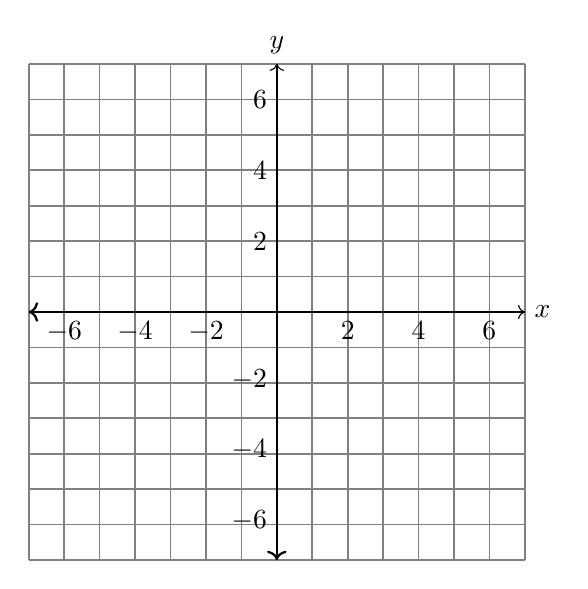
\begin{tikzpicture}[scale=.45]
\draw[help lines][semithick] (-7,-7) grid (7,7);
\draw[<-] [thick] (-7,0) -- (7,0) ;
\draw[<-] [thick] (0,-7) -- (0,7) ;
\foreach \x in {  -6, -4,  -2,  2,  4, 6 } \node[below] at (\x, 0) {$\x$};
\draw[->] (0, 0) -- (7, 0) node[right] {$x$};	% x-axis
\draw[->] (0, -7) -- (0, 7) node[above] {$y$};	% y-axis
\foreach \y/\ytext in { -5.9/-6, -3.9/-4, -1.9/-2,  2/2,4/4, 6/6} \node[left] at (0, \y) {$\ytext$};
\end{tikzpicture}
\end{parts}
\end{multicols}


 \vspace{.5cm}
\pagestyle{empty}
\hspace*{3in}{\Huge \textbf{Page 2}}

\newpage
\question   A bacteria culture starts at 2.0 billion bacteria and grows at a fixed rate.  After 8 hours there are 7.0 billion bacteria. Answer the questions below.  Notice you are asked for the exact and approximate forms of each answer.  The exact form can be found without a calculator.  This is what you will write on the exam.  If you enter your exact answer into a calculator, you get the approximate answer.  Use the exact answer from part (3.1) to do parts (3.2) and (3.3).

\begin{parts}
\part[10] Find the growth rate per hour.  (Hint: this situation can be modeled by $A(t) = A_0e^{kt}$...you are being asked to find $k$ and convert it to a percentage.)
\vfill
\begin{flushright}\fbox{%
\begin{minipage}{4 in}
Exact Answer:\hspace {1.05in} Approx. Answer\\ \hspace*{2in} (Round to 2 decimal places.):\\[4ex]

\end{minipage}}\end{flushright}
\part[10] How many billion bacteria will there be 10 hours after the start?

\vfill
\begin{flushright}\fbox{%
\begin{minipage}{4 in}
Exact Answer:\hspace {1.2in} Approx. Answer\\ \hspace*{2.15in} (Round to 1 decimal place)\\[3ex]

\hspace*{2.8in} billion bacteria
\end{minipage}}\end{flushright}
\part[10] How long will it take for the population to reach 20 billion? 

\vfill
\begin{flushright}\fbox{%
\begin{minipage}{4 in}
Exact Answer:\hspace {1.2in} Approx. Answer\\ \hspace*{2.15in} (Round to 1 decimal place)\\
\hspace*{2.15in} and write as units)\\[4ex]
\end{minipage}}\end{flushright}
\end{parts}


 \vfill
\pagestyle{empty}
\hspace*{5in}{\Huge \textbf{Page 3}}

\end{questions}


\end{document}
